\documentclass[a4paper,12pt]{article}
\usepackage{amssymb}
\usepackage{amsmath}
\usepackage[utf8]{inputenc} % Umlaute
\usepackage[ngerman]{babel} % Umlaute
\usepackage[T1]{fontenc}    % Umlaute
\usepackage[margin=2.5cm]{geometry}
\usepackage{booktabs}
\usepackage{lmodern}

% Notwendig für Links im Text
\usepackage{hyperref}

% glossar, see http://en.wikibooks.org/wiki/LaTeX/Glossary
% muss NACH hyperref geladen werden, sonst funktionieren die Links nicht
\usepackage{glossaries}

% Kompatibilität
\ifx\pdftexversion\undefined
\usepackage[dvips]{graphicx}
\else
\usepackage[pdftex]{graphicx}
\DeclareGraphicsRule{*}{mps}{*}{}
\fi

\makeglossaries

%%%%%%%%%%%%%%%%%%%%%%%%%%%%%%%%%%%%%%%%%%%%%%%%%%%%%%%%%%%%%%%%%%%%%%
% Variablen                                 						 %
%%%%%%%%%%%%%%%%%%%%%%%%%%%%%%%%%%%%%%%%%%%%%%%%%%%%%%%%%%%%%%%%%%%%%%
\newcommand{\authorName}{David Höglinger, Jan Ettrich, Erwin Müller, Benedikt Rittner, Valentin Quapil}
\newcommand{\auftraggeber}{Karlsruhe Institute of Technology (Teco)}
\newcommand{\auftragnehmer}{\authorName}
\newcommand{\projektName}{Pflichtenheft Earables}
\newcommand{\tags}{\authorName, Pflichtenheft, KIT, Informatik, PSE}
\newcommand{\glossarName}{Glossar}
\title{\projektName}
\date{\today}

%%%%%%%%%%%%%%%%%%%%%%%%%%%%%%%%%%%%%%%%%%%%%%%%%%%%%%%%%%%%%%%%%%%%%%
% PDF Meta information                                 				 %
%%%%%%%%%%%%%%%%%%%%%%%%%%%%%%%%%%%%%%%%%%%%%%%%%%%%%%%%%%%%%%%%%%%%%%
\hypersetup{
  pdfauthor   = {\authorName},
  pdfkeywords = {\tags},
  pdftitle    = {\projektName)}
}

%%%%%%%%%%%%%%%%%%%%%%%%%%%%%%%%%%%%%%%%%%%%%%%%%%%%%%%%%%%%%%%%%%%%%%
% Create a shorter version for tables. DO NOT CHANGE               	 %
%%%%%%%%%%%%%%%%%%%%%%%%%%%%%%%%%%%%%%%%%%%%%%%%%%%%%%%%%%%%%%%%%%%%%%
\newcommand\addrow[2]{#1 &#2\\ }

\newcommand\addheading[2]{#1 &#2\\ \hline}
\newcommand\tabularhead{\begin{tabular}{lp{13cm}}
\hline
}

\newcommand\addmulrow[2]{ \begin{minipage}[t][][t]{2.5cm}#1\end{minipage}%
   &\begin{minipage}[t][][t]{8cm}
    \begin{enumerate} #2   \end{enumerate}
    \end{minipage}\\ }

\newenvironment{usecase}{\tabularhead}
{\hline\end{tabular}}

\usepackage{microtype}
%%%%%%%%%%%%%%%%%%%%%%%%%%%%%%%%%%%%%%%%%%%%%%%%%%%%%%%%%%%%%%%%%%%%%%
% GLOSSARY ENTRIES                 	                              	 %
%%%%%%%%%%%%%%%%%%%%%%%%%%%%%%%%%%%%%%%%%%%%%%%%%%%%%%%%%%%%%%%%%%%%%%

\newglossaryentry{Echtzeit}{name=Echtzeit, description={Bereitstellen/Anzeigen von Daten mit einer durch die Verarbeitung bedingten Verzögerung von bis zu ca. 2 Sekunden zwischen dem Anfallen der (Roh-)Daten und der Ausgabe bzw. Visualisierung.}}
\newglossaryentry{Vorgang}{name=Vorgang, description={Als Vorgang wird in diesem Pflichtenheft bezeichnet, wenn ein Modus ausgewählt ist und Start gedrückt wurde. Der Vorgang endet mit dem Drücken von Stopp bzw. wird mit dem Wechseln des Modus.}}
\newglossaryentry{BLE}{name=BLE, description={Bluetooth Low Energy ist eine Technologie, die Teil des Industriestandards Bluetooth ist und eine energiesparende, kabellose Kommunikation zwischen Geräten in einer Entfernung von bis zu ca. 10 Metern ermöglicht.}}
\newglossaryentry{Wearable Computer}{name=Wearable Computer, description={Unter dem Begriff Wearable Computer versteht man Computersysteme, die am Körper, unter der Kleidung oder als Implantat unter der Haut getragen werden können.}}
\newglossaryentry{IMU}{name=6-Achsen IMU, description={Ein 6-Achsen IMU ist ein Beschleunigungssensor mit Gyroskop.}}
\newglossaryentry{GUI}{name=GUI, description={GUI ist die Abkürzung für den englischen Begriff \glqq graphical user interface\grqq . Sie ist die Schnittstelle zwischen Mensch und Maschine und ermöglicht dem Nutzer die Eingabe/Steuerung, der Maschine.}}
\newglossaryentry{Cross-Platform Bibliothek}{name=Cross-Platform Bibliothek, description={Eine Cross-Platform Bibliothek ist nichts weiter als eine Bibliothek die auf Rechnersystemen mit verschiedener Architektur laufen kann.}}
\newglossaryentry{Steuerungsparameter}{name=Steuerungsparameter, description={Unter Steuerungsparametern fassen wir die Länge der Verbindungsintervalle zwischen Kopfhöhrern und Handy sowie die Abtastrate und den Wertebereich von integriertem Gyroskop und Beschleunigungssensor zusammen.}}
\newglossaryentry{Schrittfrequenz}{name=Schrittfrequenz, description={Die Schrittfrequenz gibt an wie viele Schritte pro Zeiteinheit gemacht werden.}}
\newglossaryentry{Rohdaten}{name=Rohdaten, description={Als Rohdaten werden unverarbeitete Daten bezeichnet.}}
\newglossaryentry{TTS}{name=Text-To-Speech, description={Ein Text-to-Speech-System (TTS) (oder Vorleseautomat) wandelt Fließtext in eine akustische Sprachausgabe um.}}
\newglossaryentry{Earables}{name=Earables, description={Eine Zusammenschließung des Wortes Wearable und Earphone. Dabei handelt es sich um Kopfhörer, die mit Sensoren ausgestattet sind.}}
\newglossaryentry{Vorgangsdaten}{name=Vorgangsdaten, description={Daten, die bei der Ausführung eines Vorgangs gespeichert werden (z.B. Schritte, Sit-ups,\dots).}}


%%%%%%%%%%%%%%%%%%%%%%%%%%%%%%%%%%%%%%%%%%%%%%%%%%%%%%%%%%%%%%%%%%%%%%
% THE DOCUMENT BEGINS             	                              	 %
%%%%%%%%%%%%%%%%%%%%%%%%%%%%%%%%%%%%%%%%%%%%%%%%%%%%%%%%%%%%%%%%%%%%%%
\begin{document}
 \pagenumbering{roman}
 \begin{titlepage}
\maketitle
\thispagestyle{empty} % no page number

\begin{verbatim}












\end{verbatim}


  \begin{tabular}[t]{p{4 cm}p{8 cm}}
	Projekt:       & \projektName \\[1.2ex]
	Auftraggeber:  & \auftraggeber\\[1.2ex]
	Auftragnehmer: & \auftragnehmer\\[1.2ex]
  \end{tabular}


\begin{tabular}[t]{|p{4 cm}|p{8 cm}|}
\hline
\textbf{Datum} & \textbf{Autor(en)} \\
\hline
\hline
\today & \authorName \\
\hline
\end{tabular}
\end{titlepage}
         % Deckblatt.tex laden und einfügen
 \setcounter{page}{2}
 \tableofcontents          % Inhaltsverzeichnis ausgeben
 \clearpage
 \pagenumbering{arabic}

\section{Einleitung}
\Gls{Earables} gehören zu den \Gls{Wearable Computer}, sie sind also nichts anderes als intelligente Kopfhörer. Je nachdem wie sie ausgestattet werden bringen sie die unterschiedlichsten Funktionen mit sich. Neben der klassischen Ausstattung von Lautsprechern, Mikrophon und \gls{BLE} besitzen sie in unserem Fall zusätzlich eine \Gls{IMU}. Mit ihrer Hilfe ist man in der Lage die Bewegungen des Nutzers zu erkennen und aufzuzeichnen, um mit den gewonnenen Messdaten  beispielsweise die Schrittfrequenz zu messen.  \Gls{Earables} bilden also eine Schnittstelle zwischen Mensch und Computer. Da sie kaum von normalen Bluetooth Kopfhörern zu unterscheiden sind, haben sie bereits jetzt eine hohe soziale Akzeptanz in der Gesellschaft erlangt, im Gegensatz zu beispielsweise Smartglasses. Mit der Entwicklung und Forschung dieser Art von \Gls{Earables} beschäftigt sich das globale eSense Projekt von Nokia Bell Labs in Zusammenarbeit mit dem Telecooperation Office (TECO). Hier wird gemeinsam nach möglichen Anwendungsfällen der \Gls{Earables} gesucht, wodurch auch dieses Projekt initiiert wurde.
\section{Zielbestimmung}
Die Ziele dieses Projektes lassen sich in drei Bereiche gliedern:
\begin{enumerate}

  \item Es soll eine \Gls{Cross-Platform Bibliothek} (Android/IOS) für die \Gls{Earables} der Plattform eSense entwickelt werden mit der es möglich ist, die Messdaten des Gerätes aufzuzeichnen und verschiedene \Gls{Steuerungsparameter} zu verändern.
  
  \item Es soll ein Erweiterungsmodul entwickelt werden, mit dem die übermittelten  \Gls{Rohdaten} automatisch verarbeitet und ausgewertet werden, um so festzustellen ob der Nutzer gerade läuft oder steht.
  
  \item Es soll eine App mit einer \Gls{GUI} entwickelt werden, die über verschiedene Modi verfügt, insbesondere über einen der anzeigt, ob der Nutzer gerade läuft oder steht. 

\end{enumerate}

\subsection{Musskriterien}

  \begin{itemize}
    \item Die Cross-Platform Bibliothek soll in der Lage sein die gesammelten Daten der \Gls{Earables} aufzuzeichnen
    \item Die GUI der App muss so benutzerfreundlich gestaltet werden, dass der Benutzer intuitiv weiß wie man die Steuerungsparameter der \Gls{Earables} verändert
    \item Die Cross-Plattform Bibliothek soll in der Lage sein die verschiedenen Steuerungsparameter zu verändern.
    \item Das Erweiterungsmodul soll erkennen ob der Nutzer gerade \glqq läuft\grqq{}oder \glqq steht\grqq.
    \item Die App soll anzeigen können ob der Nutzer gerade läuft oder steht.
  \end{itemize}
\subsection{Wunschkriterien}
  \begin{itemize}
    \item Die App soll die \Gls{Schrittfrequenz} des Nutzers anzeigen.
    \item Die App soll die Anzahl der zurückgelegten Schritte anzeigen.
    \item Die App soll die zurückgelegte Distanz anzeigen.
    \item Die App soll über drei weitere Modi verfügen.
      \begin{itemize}
        \item\text Im Modus \glqq Zählmodus\grqq{} zählt die App wie viele Liegestützen oder Sit-ups der Nutzer macht.
        \item\text  Im Modus \glqq Lauschen\&Agieren\grqq{}kann der Nutzer seinen eigenen Trainingsplan erstellen, welcher dann über Text to Speech ausgegeben wird.
        \item\text  Im Modus \glqq Musikmodus\grqq{} wird Musik abgespielt, wenn der Nutzer läuft und automatisch pausiert, wenn der Nutzer steht. Sobald der Nutzer weiter läuft wird die Musik auch wieder weiterlaufen.
      \end{itemize}
    \item\text Im \glqq Laufmodus \grqq{} wird die aktuelle Schrittanzahl und die zurückgelegte Distanz life angezeigt.
    \item\text Die App wird standardmäßig auf Deutsch sein, als weitere Sprache steht dem Nutzer Englisch zur Auswahl.
    \item\text Trainingsdaten werden automatisch gespeichert; Importieren und Exportieren soll möglich sein.
  \end{itemize}
  \subsection{Abgrenzungskriterien}
  \begin{itemize}
    \item Es werden keine Rohdaten längerfristig gespeichert.
    \item Die Musik passt sich nicht der Schrittfrequenz des Nutzers an.
    \item Im Modus \glqq Zählen\grqq{}wird davon ausgegangen, dass der Nutzer wirklich nur Liegestützen oder Sit-ups macht. Das bewusste Austricksen des Systems durch andere Bewegungen wird nicht behandelt.
    \item Es werden nur Daten auf dem Smartphone gespeichert und nicht auf den \Gls{Earables}
  \end{itemize}

\section{Produkteinsatz}
  \subsection{Zielgruppe}
  \begin{itemize}
    \item\textsf{Bibliothek:} Softwareentwickler
    \item\textsf{Erweiterungsmodul:} Softwareentwickler
    \item\textsf{App:} Hobbysportler
  \end{itemize}
  \subsection{Anwendungsbereiche}
    \begin{itemize}
      \item\textsf{Bibliothek} Softwareentwicklung für eSense Wearables
      \item\textsf{Erweiterungsmodul} Softwareentwicklung im Bereich Schritterkennung 
      %% valle ergänzen: Vorschlag: Nutzung von Sensordaten z.B. einer App , z.b. im Fitness, aber auch als Nutzereingabe für andere interaktive Apps ? (valle)
      \item\textsf{App} Heimtraining, Sport,\dots
    \end{itemize}
  \subsection{Betriebsbedingungen der App}
    \subsection{physikalische Umgebung}
      Handy und Kopfhörer sollten nicht über zehn Meter voneinander entfernt werden, sodass eine Bluetooth-Verbindung möglich ist.
    \subsection{Sonstiges:}
      Betriebsdauer: "Akkuabhängig", keine weitere Grenzen
      Qualifikation des Benutzers: sollte Sportübungen selbstständig ausführen können
      
\section{Produktumgebung}
\subsection{Hardware} \textsf{Minimale Anforderungen:} Smartphone mit \Gls{BLE} Unterstützung.
\subsection{Software} \textsf{Betriebssystem:} Unterstützung nur von Android ab Version 7 und iOS ab Version 10.

\section{Funktionale Anforderungen}
  \subsection{Mussanforderungen}
    \subsubsection{Bibliothek}
    \begin{itemize}
      \item[/F010/] Daten des \Gls{IMU} und in \Gls{Echtzeit} zur Verfügung stellen.
      \item[/F030/] Messparameter (Abtastrate, Wertebereich Gyroskop/Beschleunigungssensor, Tiefpassfilter) ändern. 
      \item[/F040/] Datenaufnahme des \Gls{IMU} starten und stoppen.
    \end{itemize}
    \subsubsection{Erweiterungsmodul}
     Auswertung der ausgelesenen Daten:
     \begin{itemize}
      \item[/F060/] Schritterkennung (Stehen/Laufen des Nutzers).
    \end{itemize}
    \subsubsection{App}
      \begin{itemize}
      \item[/F070/] \textsf{App starten:} Der Nutzer kann die App über sein Smartphone starten. Die App startet im Laufmodus.
      \item[/F090/] \textsf{Modus wechseln:} Wechseln zwischen Modi über ein einblendebares Menü, während ein Modus ausgewählt ist.
      \item[/F100/] \textsf{Laufmodus:} Liveanzeige, ob Nutzer gerade \glqq läuft\grqq{} oder \glqq steht\grqq{}.
      \item[/F110/] \textsf{Vorgang starten:} Der Nutzer kann den modusspezifischen Vorgang starten. Dann wird der Modus nach seiner Beschreibung aktiv ausgeführt. Dies gilt für jeden Modus außer den Modus \glqq Livedaten\grqq.
      \item[/F120/] \textsf{Vorgang stoppen:} Der Nutzer kann den modusspezifischen Vorgang stoppen.
      \item[/F130/] \textsf{Resultat anzeigen:}Nach Stoppen Anzeigen des Vorgansresultats bis neuer Vorgang gestartet wird.
    \end{itemize}
  \subsection{Wunschanforderungen}
    \subsubsection{Erweiterungsmodul}
      Weitere Datenauswertung:
      \begin{itemize}
      \item[/F140/] \textsf{Schrittfrequenzerkennung}
      \item[/F150/] \textsf{Schrittzahlzähler} Zählen der Schritte des Nutzers.
      \item[/F170/] \textsf{Erkennung Sit-ups}
      \item[/F180/] \textsf{Erkennung Liegestütze}
      \end{itemize} 
    \subsubsection{App}
      Weitere Modi:
      \begin{itemize}
      \item[/F190/] \textsf{Modus Livedaten: \textit{(versteckt)}} Visualisieren der Sensorrohdaten als Graphen.
      \item[/F200/] \textsf{Zählmodus:} Zählen von Liegestützen oder Sit-ups.
      \item[/F210/] \textsf{Start/Stopp Musikmodus:} Musik stoppt wenn Nutzer stehen bleibt, läuft wenn der Nutzer läuft. Bei diesem Modus werden keine Resultate angezeigt.
      \item[/F220/]{
        Modus \glqq Lauschen\&Agieren\grqq
        \begin{itemize}
          \item[/F221/] Zusammenstellen eines Trainingsablaufs (Liegestütze, Sit-ups, Laufen). 
          \item[/F222/] Sprachanweisungen für die nächste Übung während des Trainings.
          \item[/F223/] Anzeige der Zeitdauer jeder Übung nach Ablaufsende, siehe F130.
        \end{itemize}
      }

      Einstellungen:
      \item[/F250/] Der Nutzer kann seinen Namen in den Einstellungen ändern.
      \item[/F260/] Der Nutzer kann die Sprache der App anpassen.
      \item[/F270/] Der Nutzer kann die gespeicherten \Gls{Vorgangsdaten} löschen.
      \item[/F280/] Der Nutzer kann die Steuerungsparameter anpassen. 
      \item[/F285/] Der Nutzer kann die Schrittlänge für den Modus Distanzmessung anpassen.
      
      Sonstiges:
      \item[/F290/] Aufforderung der Angabe von Name, Schrittlänge und in-App Sprache bei Erstnutzung.
      \item[/F300/] Nutzer kann in der App seine gesamten \Gls{Vorgangsdaten} exportieren und importieren.
      \item[/F310/] Speicherung der Summe der Schritte, Sit-ups und Liegestütze für jeden Tag, an dem ein Vorgang aktiv war (keine Rohdaten).
      \item[/F320/] Anzeigen der gespeicherten Daten aus /F310/
      \end{itemize}


\section{Produktdaten}
\begin{itemize}
	\item[/PD010/] Es werden keine rohen Messdaten gespeichert.
	\item[/PD020/] Die Einstellungen (Sprache, Steuerungsparameter, Messeinstellungen) sind zu speichern. 
	\item[/PD030/] Es sind relevante Daten über den Nutzer, wie den Benutzernamen, zu speichern.
	\item[/PD040/] Die \Gls{Vorgangsdaten} (Bestenliste und letzte Trainingseinheit) sind zu speichern. % Genauer definieren, was alles?
	\item[/PD050/] Speicherung aller Vorgänge, die aktiv waren mit Datum, Uhrzeit und dem letzten Resultat (/F300/)%%nächstes Treffen: abklären, ob umsetzen
	\item[/PD040/] Die Vorgangsdaten werden in der Form (Datum;Schritte;Liegestütze;Sit-ups) gespeichert. Für den Nutzer sind nur die Daten des letzten Monats aufsummiert zu sehen.
\end{itemize}


\section{Nichtfunktionale Anforderungen}
%TODO Jan Koordination

\begin{itemize}
  \item[/NF010/] Beim Ausführen der Funktion /F030/ soll die Datenaufnahme der \Gls{IMU} gestoppt werden.
  \item[/NF020/] Beim Wechseln zwischen Modi (/F090/) soll der aktuelle Modus terminiert werden.
  \item[/NF030/] Nach Ausführung der Funktion  Sprachänderung (/F260/) muss die App neu gestartet werden.
  \item[/NF040/] Bei nicht sinnvollen Angaben (z.B. negativen Werten in /F220/) wird das Starten des Vorgangs verhindert.
  \item[/NF050/] Bei Namensänderung (/F250/) werden gespeicherte Daten (siehe ev. /F300/) nicht verändert.
  \item[/NF060/] Bei Namensgebung sind nur Groß- und Kleinbuchstaben ohne Umlaute und Sonderzeichen erlaubt.
\end{itemize}
\subsection{Stabilität}
\begin{itemize}
  \item[/NF070/] Die App soll bei herkömmlicher Nutzung nicht öfter als zweimal bei zehnmaliger Benutzung. %stabilität
\end{itemize}
\subsection{Speicherplatz}
\begin{itemize}
  \item[/NF080/] Die App soll eine Größe von 100 MByte nicht überschreiten. %speicher
  \item[/NF090/] Die gespeicherten Daten sollen nicht mehr als 50 MByte umfassen. %speicher] 
\end{itemize}
\subsection{Laufzeitverhalten}
\begin{itemize}
  \item[/NF100/] Die Funktionen /F060/ und /F100/ (Laufmodus) soll maximal eine Verzögerung von zwei Sekunden aufweisen. %%Laufzeitverhalten
  \item[/NF110/] Der Start eines Modus nach seiner Auswahl (/F080/) soll nicht länger als zwei Sekunden benötigen. %%Laufzeitverhalten] 
  \item[/NF120/] Die Einblendung des Vorgangsresultats (/F130/) soll nicht länger als zwei Sekunden benötigen.%%Laufzeitverhalten

\end{itemize}
\section{Systemmodelle}
%%TODO Jan!!
  \subsection{Architekturdiagramm}
  \begin{center}
  	\vspace{100px}
  	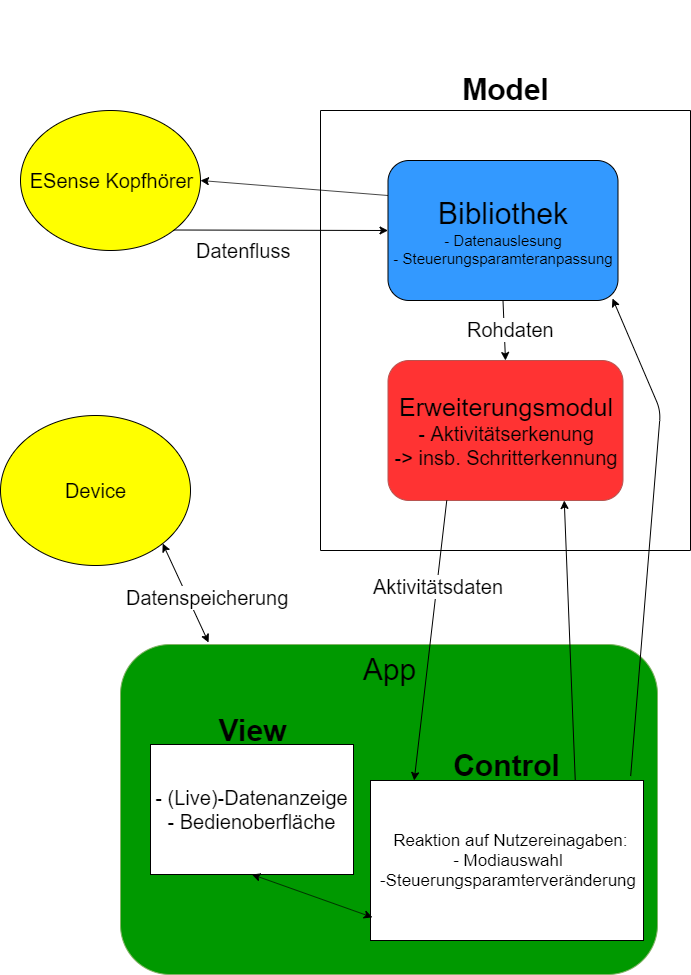
\includegraphics[width=0.8\textwidth]{NeuesArchitekturdiagramm.png}
  \end{center}
  
  \subsection{Use-Case-Diagramm}
  \begin{center}
	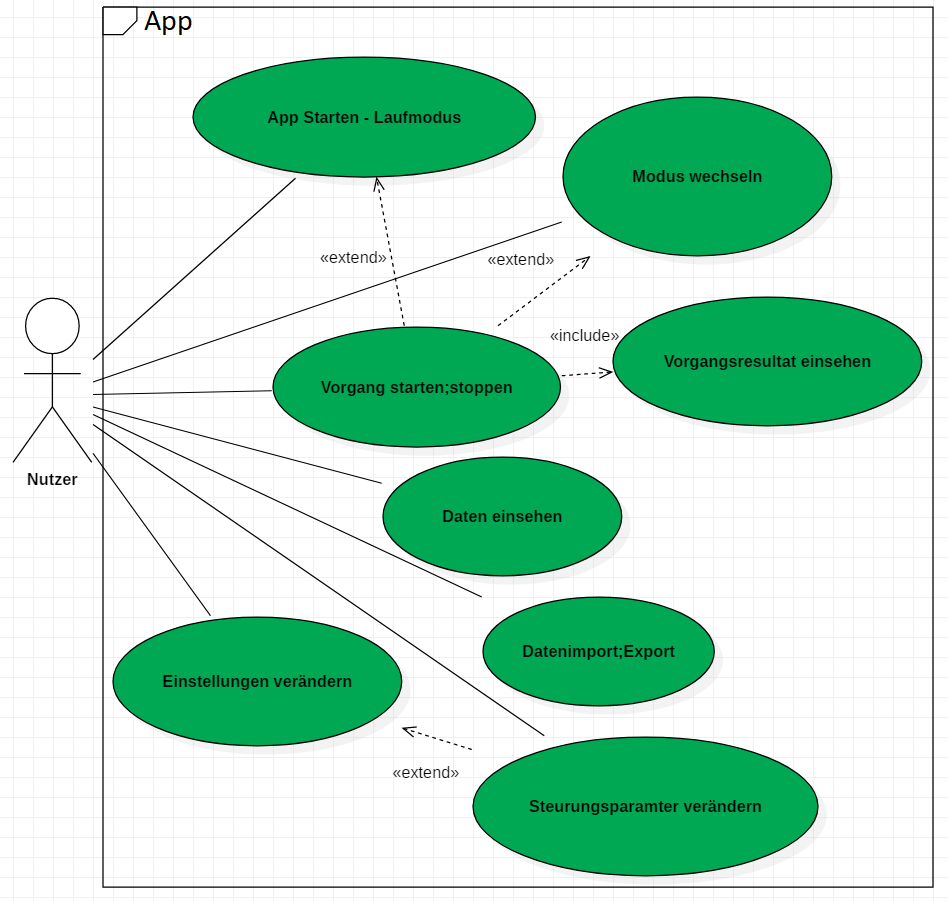
\includegraphics[width=0.8\textwidth]{Use-CaseDiagramm.png} 
  \end{center}

Kurzbeschreibung: Beim Starten der App durch den Nutzer startet automatisch der Laufmodus. Der Nutzer kann nun entweder den Modus wechseln oder einen Vorgang starten. Nach Beendigung oder Stoppen des Vorgangs wird das Vorgangsresultat angezeigt. Der Nutzer kann außerdem die Vorgangsdaten des letzten Monats einsehen und seine Daten importieren/exportieren. Das Ändern von Einstellungen und der damit verbundenen Steuerungsparameter der \Gls{Earables} ist ebenfalls möglich.
\section{Benutzeroberfläche}
Die \Gls{GUI} wird durch die App realisiert. Dabei kann man die einzelnen Modi über das Navigationsmenü auswählen. Jeder Modus hat zwei Seiten; eine Übersichtsseite und eine aktive Seite, welche während des aktiven \Gls{Vorgang} angezeigt wird. Für die weiteren Funktionen(Einstellungen, Dateienexport/-import) bietet die Applikation ebenfalls spezielle Seiten an.
Die \Gls{GUI} kann getestet werden mithilfe des Design-Tools \glqq Mock-up\grqq{} über den angegebenen Link in der Fußnote \footnote[1]{Mock-Up Prototyp: https://app.moqups.com/448nRiafse/view/page/a70dc1e41?ui=0}


\begin{figure}[ht!]
	\centering

	
		\begin{minipage}{0.4\textwidth}
			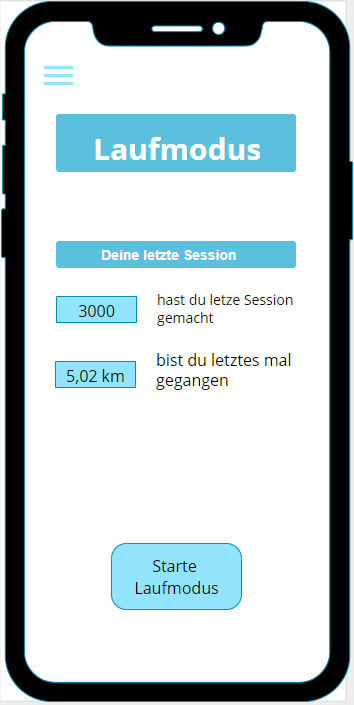
\includegraphics[width=4cm,height=9cm]{./Benutzeroberflaeche/Laufmodus.png}
			\caption{Laufmodus}
			\vspace{30px}
		\end{minipage}
			\hfill
		\begin{minipage}{0.4\textwidth}
			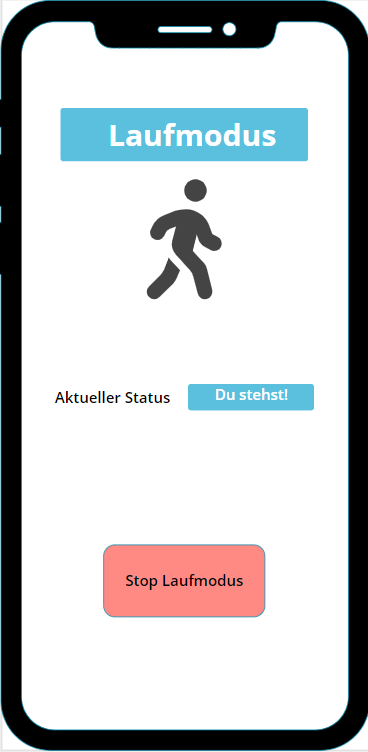
\includegraphics[width=4cm,height=9cm]{./Benutzeroberflaeche/Laufmodus_aktiv.png}
			\caption{aktiver Laufmodus}
			\vspace{30px}
		\end{minipage}
		\begin{minipage}{0.4\textwidth}
			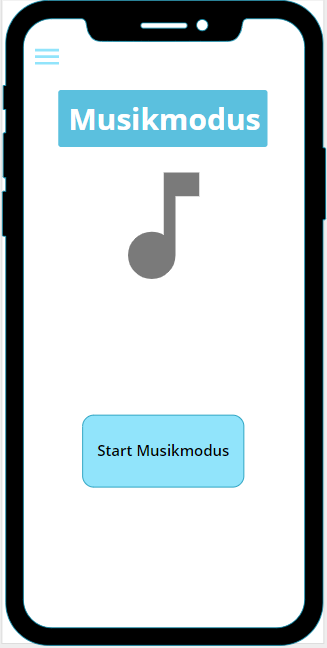
\includegraphics[width=4cm,height=9cm]{./Benutzeroberflaeche/Musikmodus.png}
			\caption{Musikmodus}
		\end{minipage}
		\hfill
		\begin{minipage}{0.4\textwidth}
			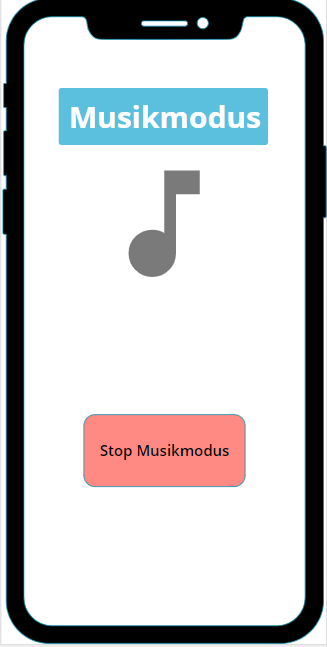
\includegraphics[width=4cm,height=9cm]{./Benutzeroberflaeche/Musikmodus_aktiv.png}
			\caption{aktiver Musikmodus}
			
		\end{minipage}
\end{figure}

\begin{figure}[ht!]
	
	\centering
	\begin{minipage}{0.4\textwidth}
		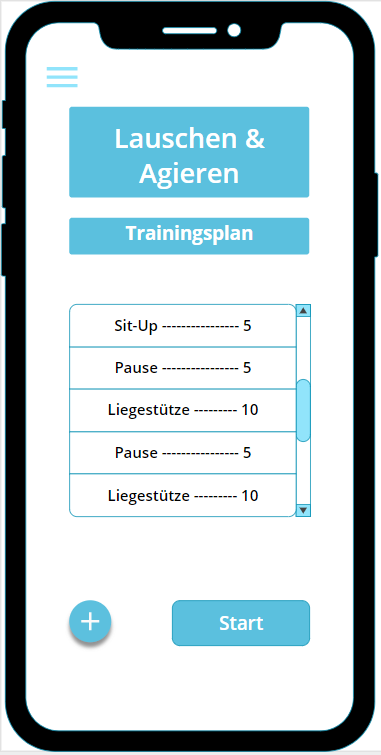
\includegraphics[width=4cm,height=9cm]{./Benutzeroberflaeche/Lauschen_und_Agieren.png}
		\caption{Lauschen und Agieren}
		\vspace{30px}
	\end{minipage}
	\hfill
	\begin{minipage}{0.4\textwidth}
		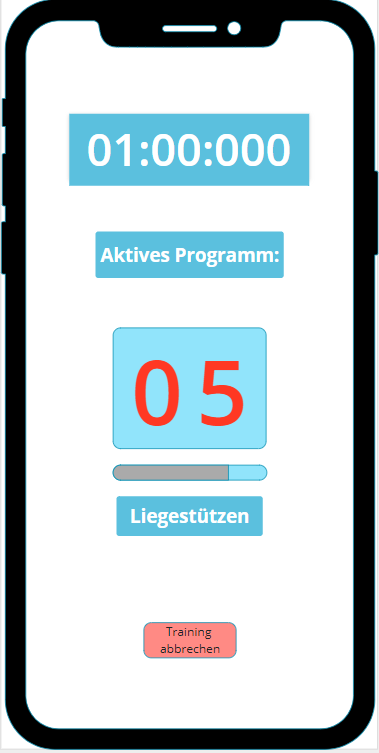
\includegraphics[width=4cm,height=9cm]{./Benutzeroberflaeche/Lauschen_und_Agieren_aktiv.png}
		\caption{Lauschen und Agieren aktiv}
		\vspace{30px}
	\end{minipage}
	\begin{minipage}{0.4\textwidth}
		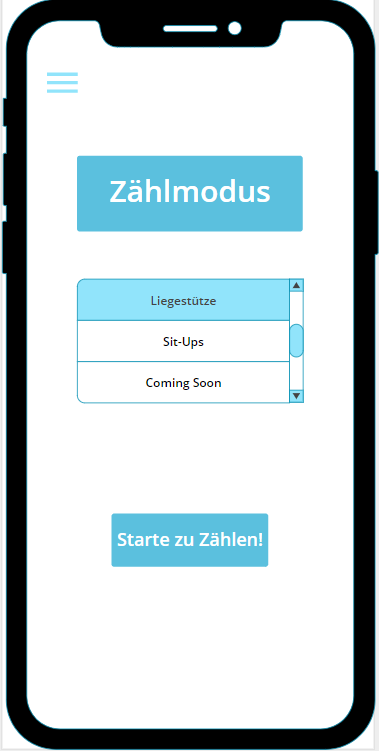
\includegraphics[width=4cm,height=9cm]{./Benutzeroberflaeche/Zaehlmodus.png}
		\caption{Zählmodus}		
	\end{minipage}
	\hfill
	\begin{minipage}{0.4\textwidth}	
		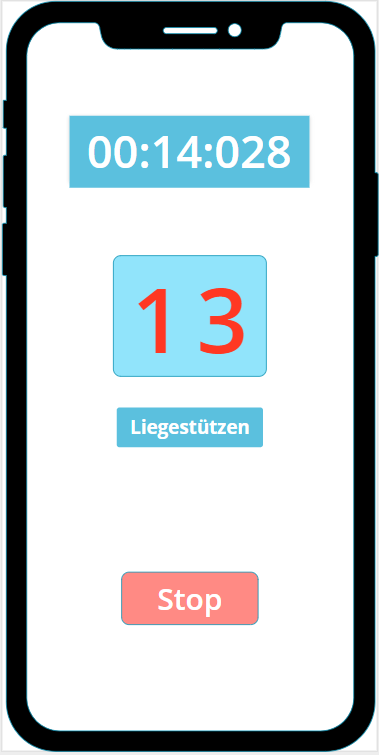
\includegraphics[width=4cm,height=9cm]{./Benutzeroberflaeche/Zaehlmodus_aktiv.png}
		\caption{Zählmodus aktiv}
		
	\end{minipage}
\end{figure}
\begin{figure}[ht!]
	\centering
	\begin{minipage}{0.4\textwidth}
		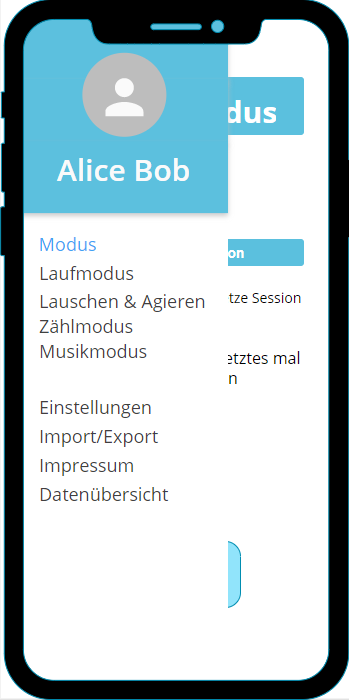
\includegraphics[width=4cm,height=9cm]{./Benutzeroberflaeche/Sidemenu.png}
		\caption{Navigationsmenü}
		\vspace{30px}
	\end{minipage}
	\hfill
	\begin{minipage}{0.4\textwidth}
		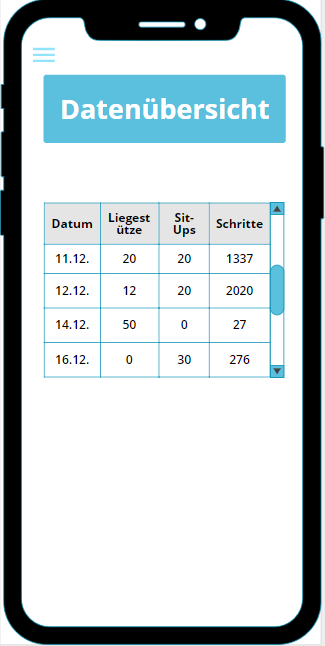
\includegraphics[width=4cm,height=9cm]{./Benutzeroberflaeche/Datenuebersicht.png}
		\caption{Datenübersicht}
		\vspace{30px}
	\end{minipage}
	\begin{minipage}{0.4\textwidth}
		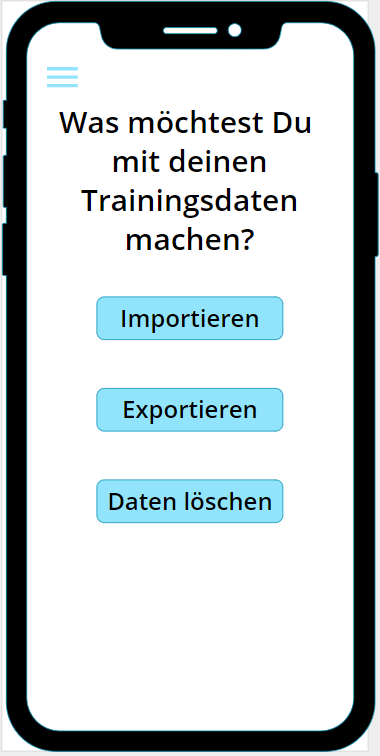
\includegraphics[width=4cm,height=9cm]{./Benutzeroberflaeche/Import_Export.png}
		\caption{Import und Export}
	\end{minipage}
	\hfill
	\begin{minipage}{0.4\textwidth}
		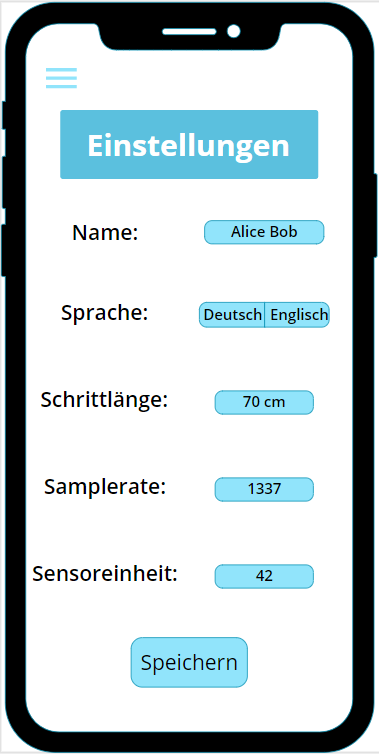
\includegraphics[width=4cm,height=9cm]{./Benutzeroberflaeche/Settings.png}
		\caption{Einstellungen}
	\end{minipage}
\end{figure}
\newpage
\clearpage

\section{Qualitätszielbestimmungen}
\begin{tabular}[t]{|c|c|c|c|c|c|}
  \hline
  \textbf{Kriterium} & \textbf{Sehr Wichtig} & \textbf{Wichtig} & \textbf{Weniger Wichtig} & \textbf{Unwichtig}\\
  \hline
  \hline
  Korrektheit & x & & &\\ %%sehr
  \hline
  Zuverlässigkeit & & x & &\\ %%weniger
  \hline
  Robustheit & & & x &\\  %%weniger
  \hline
  Effizienz & & x & &\\ %%wichtig
  \hline
  Benutzerfreundlichkeit & x & & &\\ %%sehr
  \hline
  Vertrauenswürdigkeit & & & x &\\ %%un
  \hline

\end{tabular}

 %%!! Was ist hiermit? Stand noch in der Mail als Unterpunkt. https://www.sosy-lab.org/Teaching/2015-WS-SEP/samples/pflichtenheft.pdf Seite 13 sieht man so eine Tabelle, wie ist das gemeint?
 %%nächstes Treffen: ***kurzes*** Planungspoker mit Korrektheit, Zuverlässigkeit, Robustheit, Effizienz, Benutzerfreundlichkeit und Vertrauenswürdigkeit zwischen sehr wichtig, wichtig, weniger wichtig und unwichtig.
 %% code-standards??
\section{Globale Testfälle und Szenarien}
%%TODO David
  \subsection{Globale Testfälle}
  \subsubsection{Bibliothek}
  \begin{itemize}
    \item[/T010/] Die Bibliothek kann die Daten des \Gls{IMU} in \Gls{Echtzeit} zur Verfügung stellen.
    \item[/T030/] Mithilfe der Bibliothek lassen sich (Abtastrate, Wertebereich Gyroskop/Beschleunigungssensor, Tiefpassfilter) ändern. 
    \item[/T040/] Die Bibliothek erlaubt es die Datenaufnahme des \Gls{IMU} zu starten und zu stoppen.
  \end{itemize}
  \subsubsection{Erweiterungsmodul}
  \begin{itemize}
    \item[/T060/] Das Erweiterungsmodul erkennt Schritte.
  \end{itemize}
  \subsubsection{App}
    \begin{itemize}
    \item[/T070/] Der Nutzer kann die App über sein Smartphone starten. Die App startet im Laufmodus.
    \item[/T090/] Der Nutzer kann die Modi über ein einblendebares Menü wechseln, während ein Modus ausgewählt ist.
    \item[/T100/] Der Nutzer kann sehen, ob er gerade \glqq läuft\grqq{} oder \glqq steht\grqq{}.
    \item[/T110/] Der Nutzer kann den modusspezifischen Vorgang starten. Dann wird der Modus nach seiner Beschreibung aktiv ausgeführt. Dies gilt für jeden Modus außer den Modus \glqq Livedaten\grqq.
    \item[/T120/] Der Nutzer kann den modusspezifischen Vorgang stoppen.
    \item[/T130/] Die App zeigt nach Stoppen des Vorgangs das Vorgansresultats an bis neuer Vorgang gestartet wird.
  \end{itemize}
\subsection{Wunschanforderungen}
  \subsubsection{Erweiterungsmodul}
    \begin{itemize}
    \item[/T140/] Ermittelt die aktuelle Schrittfrequenz korrekt.
    \item[/T150/] Zählt die Schritte des Nutzers.
    \item[/T170/] Erkennt Sit-ups.
    \item[/T180/] Erkennt Liegestütze.
  \end{itemize}
  \subsubsection{App}
  \begin{itemize}
    \item[/T190/] Die Sensorrohdaten werden als Graphen angezeigt.
    \item[/T200/] Die Liegestützen oder Sit-ups werden von der App gezählt.
    \item[/T210/] Musik stoppt wenn Nutzer stehen bleibt, läuft wenn der Nutzer läuft.
    \item[/T221/] Einen Trainingsplan zusammenstellen.
    \item[/T222/] Die App gibt dem Nutzer über Sprachanweisung aus was die nächste Übung ist.
    \item[/T223/] Nach der Übung wird die benötigte Zeit angezeigt.
    \item[/T250/] Der Nutzer ändert seinen Namen.
    \item[/T260/] Der Nutzer ändert die Sprache.
    \item[/T270/] Trainingsdaten löschen.
    \item[/T280/] Die Samplingrate verändern.
    \item[/T285/] Die Schrittlänge verändern.
    \item[/T290/] Bei der Erstnutzung wird der Nutzer aufgefordert seinen Namen, seine Schrittlänge und die Sprache zu setzen.
    \item[/T300/] Trainingsdaten importieren und exportieren.
    \item[/T320/] Die gespeicherten Trainingsdaten ansehen.
   \end{itemize}
   
  \subsection{Szenarien}
    \subsubsection{Mussanforderungen}
      \paragraph{Laufmodus (/T100/)}
      \begin{enumerate}
        \item Das Smartphone wird per Bluetooth mit den Kopfhörern verbunden.
        \item Der Nutzer startet die App.
        \item Nach dem Startvorgang der App wird in den Modus \glqq Laufmodus\grqq{} gewechselt.
        \item Die Kopfhörer werden korrekt am Ohr des Nutzers angebracht.
        \item Die App zeigt dem Nutzer den Status \glqq stehend\grqq{} an.
        \item Sobald der Nutzer anfängt zu gehen zeigt die App \glqq gehend\grqq{} an.
        \item Sobald der Nutzer wieder still steht ändert sich der Zustand wieder zurück zu \glqq stehend\grqq. 
      \end{enumerate}

    \subsubsection{Wunschanforderungen}
        
    \paragraph{Livedaten (/F190/)}
      \begin{enumerate}
        \item Das Smartphone wird per Bluetooth mit den Kopfhörern verbunden.
        \item Der Nutzer startet die App.
        \item Nach dem Startvorgang der App wechselt der Nutzer in den Modus \glqq Livedaten\grqq . (/F190/)
        \item Die Kopfhörer werden korrekt am Ohr des Nutzers angebracht.
        \item Der Nutzer startet den gewählten Vorgang.
        \item Die App zeigt die korrekten Sensordaten an. (/T190/)
      \end{enumerate}

    
    \paragraph{Zählmodus (/F200/)}
      \begin{enumerate}
        \item Das Smartphone wird per Bluetooth mit den Kopfhörern verbunden.
        \item Der Nutzer startet die App.
        \item Nach dem Startvorgang der App wechselt der Nutzer in den Modus \glqq Zählmodus\grqq . (/F200/)
        \item Die Kopfhörer werden korrekt am Ohr des Nutzers angebracht.
        \item Der Nutzer wählt eine verfügbare Übung aus. 
        \item Der Nutzer startet den gewählten Vorgang.
        \item Der Nutzer führt die Übung X (natürliche Zahl) mal aus.
        \item Der Nutzer stoppt den laufenden Vorgang.
        \item Die App zeigt X an. (/T200/)
      \end{enumerate}

    
    \paragraph{Start/Stop Musikmodus (/F210/)}
      \begin{enumerate}
        \item Das Smartphone wird per Bluetooth mit den Kopfhörern verbunden.
        \item Der Nutzer spielt Musik mit der vorinstallierten Musik-App ab.
        \item Der Nutzer startet die App.
        \item Nach dem Startvorgang der App wechselt der Nutzer in den Modus \glqq Laufmodus\grqq . (/F210/)
        \item Die Kopfhörer werden korrekt am Ohr des Nutzers angebracht.
        \item Der Nutzer beginnt zu gehen.
        \item Der Nutzer startet den gewählten Vorgang.
        \item Der Nutzer hört auf zu gehen.
        \item Die Musik wird pausiert. (/T210/)
        \item Der Nutzer geht weiter.
        \item Die Musik startet automatisch wieder. (/T210/)
      \end{enumerate}
  
      \paragraph{Lauschen\&Agieren (/F220/)}
      \begin{enumerate}
        \item Das Smartphone wird per Bluetooth mit den Kopfhörern verbunden.
        \item Der Nutzer startet die App.
        \item Nach dem Startvorgang der App wechselt der Nutzer in den Modus \glqq Lauschen\&Agieren\grqq . (/F220/)
        \item Die Kopfhörer werden korrekt am Ohr des Nutzers angebracht.
        \item Der Nutzer stellt sich ein Training aus den verfügbaren Übungen zusammen (/T221/).
        \item Der Nutzer startet den gewählten Vorgang.
        \item Dem Nutzer wird per \Gls{TTS} die aktuelle Übung angesagt (/T222/).
        \item Der Nutzer führt die Übung aus.
        \item Die letzten beiden Schritte werden so lange wiederholt, bis alle ausgewählten Übungen erledigt sind.
        \item Der Vorgang wird automatisch beendet.
        \item Die App zeigt die benötigten Zeiten pro Übung an (/T223/).
      \end{enumerate}

      \paragraph{Einstellungen (TF250/ bis /T285/)}
      \textit{Voraussetzung: /T220/}
      \begin{enumerate}
        \item Das Smartphone wird per Bluetooth mit den Kopfhörern verbunden.
        \item Der Nutzer startet die App.
        \item Nach dem Startvorgang der App wechselt der Nutzer in die Ansicht \glqq Einstellungen\grqq .
        \item Der Nutzer ändert seinen Namen (/T250/).
        \item Der Nutzer ändert die Sprache (/T260/).
        \item Dem Nutzer löscht die gespeicherten \Gls{Vorgangsdaten} (/T270/).
        \item Dem Nutzer ändert die Steuerungsparameter (/T280/).
        \item Der Nutzer ändert seine Schrittlänge (/T285/).
        \item Der Nutzer beendet die App.
        \item Der Nutzer startet die App.
        \item Der Nutzer wechselt in die Ansicht \glqq Einstellungen\grqq .
        \item Die Einstellungen sind exakt so, wie sie vorher eingestellt wurden.
      \end{enumerate}

      \paragraph{Erstnutzung (/T290/)}
      \begin{enumerate}
        \item Der Nutzer startet die App zum ersten Mal.
        \item Der Nutzer wird aufgefordert seinen Namen, seine Schrittlänge und die in-App Sprache zu setzen.
        \item Danach wechselt die App in den \glqq{}Laufmodus \grqq{}.
        \item Der Nutzer schließt die App.
        \item Der Nutzer startet die App erneut und befindet sich nun im \glqq{}Laufmodus\grqq.
        \item Sein Name, seine Schrittlänge und die in-App Sprache wurden gespeichert.
      \end{enumerate}

      \paragraph{Vorgangsdaten importieren/exportieren (/T300/)}


\section{Entwicklungsumgebung}
Wir arbeiten an dem Projekt mit Visual Studio 2019, sodass alle eine einheitliche Entwicklungsumgebung verwenden.\\
Dabei kommt der .NET Standard 2.0 zum Einsatz, der C\# 7.2 verwendet. Wir arbeiten außerdem mit Xamarin Forms.\\
Zur Versionskontrolle und zur Projektübersicht wird Git verwendet, das Repository liegt öffentlich auf Github\footnote{\url{https://github.com/vlle1/earablesKIT}}.
\clearpage
\printglossaries
\stepcounter{section}
\end{document}
